%%%%%%%%%%%%%%%%%%%%%%%%%%%%%%%%%%%%%%%%%%%%%%%%%%%%%%%%%%%%%%%%%%%%%%
% How to use writeLaTeX: 
%
% You edit the source code here on the left, and the preview on the
% right shows you the result within a few seconds.
%
% Bookmark this page and share the URL with your co-authors. They can
% edit at the same time!
%
% You can upload figures, bibliographies, custom classes and
% styles using the files menu.
%
% If you're new to LaTeX, the wikibook is a great place to start:
% http://en.wikibooks.org/wiki/LaTeX
%
%%%%%%%%%%%%%%%%%%%%%%%%%%%%%%%%%%%%%%%%%%%%%%%%%%%%%%%%%%%%%%%%%%%%%%
\documentclass{tufte-handout}
%\usepackage{thmtools}

%\geometry{showframe}% for debugging purposes -- displays the margins

\usepackage{amsmath}

% Set up the images/graphics package
\usepackage{graphicx}
\setkeys{Gin}{width=\linewidth,totalheight=\textheight,keepaspectratio}
\graphicspath{{graphics/}}

\title[Lecture 1a]{\large EE2100/EE5609 Matrix Theory \\ \LARGE Lecture 1a: Basis and dimension}
\author[Aditya S]{Scribe(s): Aditya Siripuram}
\date{\today}  % if the \date{} command is left out, the current date will be used

% The following package makes prettier tables.  We're all about the bling!
\usepackage{booktabs}
\usepackage{amsmath, amsthm, amssymb, bm}
\usepackage{tikz, pgfplots}
\usetikzlibrary{shapes, arrows, positioning, fit, calc}   
\tikzset{block/.style={draw, thick, text width=1.2cm ,minimum height=0.8cm, align=center},   
line/.style={-latex}     
} 

\newtheorem{theorem}{Theorem}
\theoremstyle{remark}
\newtheorem*{defn}{Definition}
\renewcommand{\vec}[1]{\underline{#1}}
% The units package provides nice, non-stacked fractions and better spacing
% for units.
\usepackage{units}

% The fancyvrb package lets us customize the formatting of verbatim
% environments.  We use a slightly smaller font.
\usepackage{fancyvrb}
\fvset{fontsize=\normalsize}

% Small sections of multiple columns
\usepackage{multicol}

% Provides paragraphs of dummy text
\usepackage{lipsum}

% These commands are used to pretty-print LaTeX commands
\newcommand{\doccmd}[1]{\texttt{\textbackslash#1}}% command name -- adds backslash automatically
\newcommand{\docopt}[1]{\ensuremath{\langle}\textrm{\textit{#1}}\ensuremath{\rangle}}% optional command argument
\newcommand{\docarg}[1]{\textrm{\textit{#1}}}% (required) command argument
\newenvironment{docspec}{\begin{quote}\noindent}{\end{quote}}% command specification environment
\newcommand{\docenv}[1]{\textsf{#1}}% environment name
\newcommand{\docpkg}[1]{\texttt{#1}}% package name
\newcommand{\doccls}[1]{\texttt{#1}}% document class name
\newcommand{\docclsopt}[1]{\texttt{#1}}% document class option name

\begin{document}

\maketitle% this prints the handout title, author, and date
\fancyhead[L]{EE2100/EE5609}
%\begin{abstract}
%\noindent This document describes the Tufte handout \LaTeX\ document style.
%It also provides examples and comments on the style's use.  Only a brief
%overview is presented here; for a complete reference, see the sample book.
%\end{abstract}

%\printclassoptions
\begin{itemize}
    \item These notes are purposefully terse; you can generate more detailed notes, as per your writing style.
    \item Include a short summary of the concepts covered so far (in particular if they relate to the topic you are writing about)
\end{itemize}
\newthought{Recall:} vector spaces, matrix multiplication, linear independence
\section{Basis and dimension}\marginnote{ For example, the set \( \left\{\begin{pmatrix}1 \\ 0 \\ 0 \end{pmatrix}, \begin{pmatrix}1 \\ 1 \\ 0 \end{pmatrix}, \begin{pmatrix}1 \\ 1 \\ 1 \end{pmatrix}   \right\}\) is a basis for $\mathbb{R}^3$. The set $\{1, x, x^2, x^3 \}$ is a basis for the vector space consisting of all degree $3$ polynomials, etc.}
A maximal linearly independent set in a vector space is called a basis. We say that a set $T \subseteq \mathcal{V}$ is maximally linearly independent if adding any vector to $T$ makes it linearly dependent, i.e. 
\[
T\cup \{\vec{v}\} \text{ is linearly dependent  for any }\vec{v} \in \mathcal{V}.
\]


\begin{theorem}
If $\{\vec{v}_1, \vec{v}_2, \ldots, \vec{v}_k\}$ is a basis for $\mathcal{V}$, then every vector $\vec{v} \in \mathcal{V}$ can be written uniquely as \marginnote{This result highlights the importance of a basis. There are two aspects to this theorem: First that any vector \emph{can} be expressed as a linear combination of the vectors in the basis, and secondly, that such an expression is \emph{unique}. This justifies the term `basis': a set that can be used to build the vector space.}
\[
\vec{v} = \sum_{i=1}^k \alpha_i \vec{v}_i.
\]
\end{theorem}
The scalars $\alpha_i$ are called the coefficients or coordinates of the vector $\vec{v}$ in the given basis.
\begin{proof}

\begin{enumerate}
    \item \emph{Span:} Suppose we have a $\vec{v} \in \mathcal{V}$ that cannot be written as a linear combination of $\{\vec{v}_1, \vec{v}_2, \ldots, \vec{v}_k\}$. Then $\vec{v} \cup \{\vec{v}_1, \vec{v}_2, \ldots, \vec{v}_k\}$ is a linearly independent set (why?), contradicting of maximality of $\{\vec{v}_1, \vec{v}_2, \ldots, \vec{v}_k\}$.
    \item \emph{Uniqueness:} Suppose there are two different ways of writing $\vec{v}$ as a linear combination
    \[
    \vec{v} = \sum_{i=1}^k \alpha_i \vec{v}_i , \quad \vec{v} = \sum_{i=1}^k \beta_i \vec{v}_i, \text{ with } (\alpha_1, \alpha_2, \ldots) \neq (\beta_1, \beta_2, \ldots). 
    \]
    Then  $\sum_{i=1}^k (\alpha_i - \beta_i) \vec{v}_i = 0$, giving a non-trivial linear combination that is zero. This contradicts the linear independence of $\{\vec{v}_1, \vec{v}_2, \ldots, \vec{v}_k\}$.
\end{enumerate}
\end{proof}

There could be many bases for a vector space \footnote{As an excercise, try to construct three different bases for $\mathbb{R}^3$}. The following result guarantees that all bases of a vector space have the same number of elements.

\begin{theorem}
\label{thm:dim}
\marginnote{Since all bases (maximally linearly independent sets) have the same size, one could also have defined a basis as a \emph{maximum} size linearly independent set.} Any two bases of a vector space have the same number of elements.
\end{theorem}

\begin{proof}
Suppose we have bases $\{\vec{v}_1, \vec{v}_2, \ldots, \vec{v}_k \}$ and $\{\vec{w}_1, \vec{w}_2, \ldots, \vec{w}_p \}$ with $k < p$. Let \(V = \begin{pmatrix} \vec{v}_1 & \vec{v}_2 & \ldots & \vec{v}_k \end{pmatrix}\) and \(W = \begin{pmatrix} \vec{w}_1 & \vec{w}_2 & \ldots & \vec{w}_p \end{pmatrix}\) be the corresponding matrices. Then $W = V A$ for some $k \times p$ matrix $A$ (why ? \footnote{This is obtained by writing each basis vector in $\{\vec{w}_1, \vec{w}_2, \ldots, \vec{w}_p \}$ in terms of the basis vectors in $\{\vec{v}_1, \vec{v}_2, \ldots, \vec{v}_k \}$.}). Thus the linear independence of columns of $W$ and columns of $V$ implies that 
\[
A\vec{x} = 0 \text{ only when } \vec{x}=0,
\]
which is a contradiction since $A$ is a fat matrix ($k<p$) \footnote{This result (that $A\vec{x}=0$ always has a non zero solution when $A$ is fat) was used in an earlier lecture as well. We can prove it using row echelon forms, which we will defer till later in the course.}.
\end{proof}
Because of Theorem \ref{thm:dim}, it makes sense to define the following:

\begin{defn}
\newthought{The dimension} of a vector space is the size of any basis in the vector space. \sidenote{What is the dimension of  the set of all degree 3 polynomials $f$ with $f(0) = 0$? You need to first check that this is a vector space. }
\end{defn}


\section{Matrix spaces}
Recall the system interpretation of a matrix. In view of that, we define the following \begin{marginfigure}
\begin{center}
    

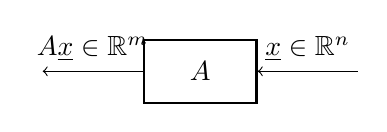
\begin{tikzpicture}  
  \node[block] (a) {$A$};  
  \draw[->] (2,0) -- node[above]{$\vec{x} \in \mathbb{R}^n$}
  (a);
  \draw[->] (a) -- node[above]{$A\vec{x} \in \mathbb{R}^m$} (-2,0);
\end{tikzpicture}  
\end{center}
\caption{System interpretation of an $m \times n$ matrix $A$. The matrix takes an `input' $\vec{x} \in \mathbb{R}^n$ and gives an `output' $A \vec{x} \in \mathbb{R}^m$. The input space is $\mathbb{R}^n$ and the output space is $\mathbb{R}^m$.}
\end{marginfigure}

\begin{enumerate}
    \item The image space of $A$, written $im(A)$  \footnote{Note that $im(A)$ lies in the output space, i.e. $im(A) \subseteq \mathbb{R}^m$. Since $A\vec{x}$ is a linear combination of columns of $A$, the set $im(A)$ is also called the column space of $A$.}is the set of all possible outputs of $A$
    \[
    im(A) = \{A\vec{x}: \vec{x} \in \mathbb{R}^n\}.
    \] 
    \item The null space of $A$, written $null(A)$  \footnote{Note that $null(A)$ lies in the input space, i.e. $null(A) \subseteq \mathbb{R}^n$.},is the set of all inputs that give a zero output
    \[
     null(A) = \{\vec{x}  \in \mathbb{R}^n : A\vec{x}= 0\}.
    \]
Characterize the column and null spaces of \[
A = \begin{pmatrix} 1 & 1 \\ 1 & 1 \end{pmatrix} \quad B = \begin{pmatrix} 1 & 2 \\ 2 & 4 \end{pmatrix}.
\]
\begin{marginfigure}
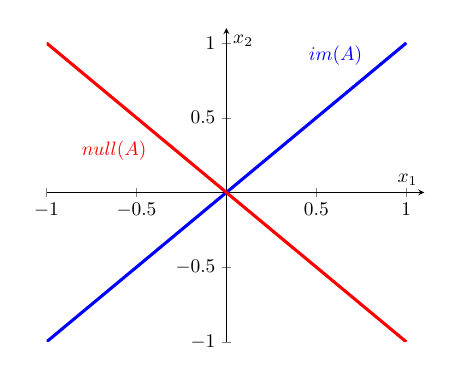
\begin{tikzpicture}[scale=0.7]
    \begin{axis}[
        axis lines=center,
        xmax = 1.1,
        ymax = 1.1,
        ylabel=$x_2$,
        xlabel=$x_1$,
        ]
        \addplot [domain=-1:1,samples=250, ultra thick, blue] {x}
            node [pos=0.9, above left] {$im(A)$};
        \addplot [domain=-1:1,samples=250, ultra thick, red ] {-x}
            node [pos=0.3, below left] {$null(A)$};
    \end{axis}
        \end{tikzpicture}
\caption{For the $2 \times 2$ matrix $A$, both $im(A)$ and $null(A)$ are in $\mathbb{R}^2$, plotted above. Verify, and similarly repeat for $B$.}
\end{marginfigure}
\end{enumerate}


%\bibliography{references}
%\bibliographystyle{plainnat}



\end{document}